\clearpage
\chapter{\textbf{Implementation}}\label{Implementation}
\subsubsection{Sewing Machine Signal Connection and Data Acquisition}
The final signals necessary to calculate all selected KPIs are "Thread Trimming," "Pressure foot," "Upper shaft rotating," and "Main menu and not sewing." The retrieval of these signals was contingent upon their initial assignment to the correct output pins in the machine's menu configuration. The subsequent challenge was to establish a connection between the output pins and the input pins of the WAGO PLC.

A connection for one signal from the sewing machine had already been established during an earlier project, but unfortunately, the connection was inadequately documented. This proved to be more confusing than helpful. The connection was implemented as follows: The signal pin of the sewing machine was connected to the 0V reference of the PLC. The 24V pin of the sewing machine was connected to the signal input connector of the PLC. Figure 5.1 provides a visual aid to facilitate comprehension of this configuration. This arrangement made sense once it was discovered that the sewing machine signals are NPN type, while the PLC exclusively accepts PNP signals as input. Typically, when the sewing machine would also have signals of type PNP, the signal pins would simply be connected to the signal connectors of the PLC. Concurrently, the 0V connector of the PLC would be connected to the GND pin of the sewing machine.

The system was configured so that when a signal becomes active, it draws current through the signal input connector of the PLC, resulting in a high signal. However, this implementation was limited to only two signals, because there is only one 0V connector available for two signal input connectors. In total, there are two 0V connectors and four signal input connectors. When two 24V pins are connected to one 0V connector via the signal input pins, an active signal draws current through the 0V connection and simultaneously pulls current from both input signal connectors. This results in invalid signals. 
\begin{figure}[H]
	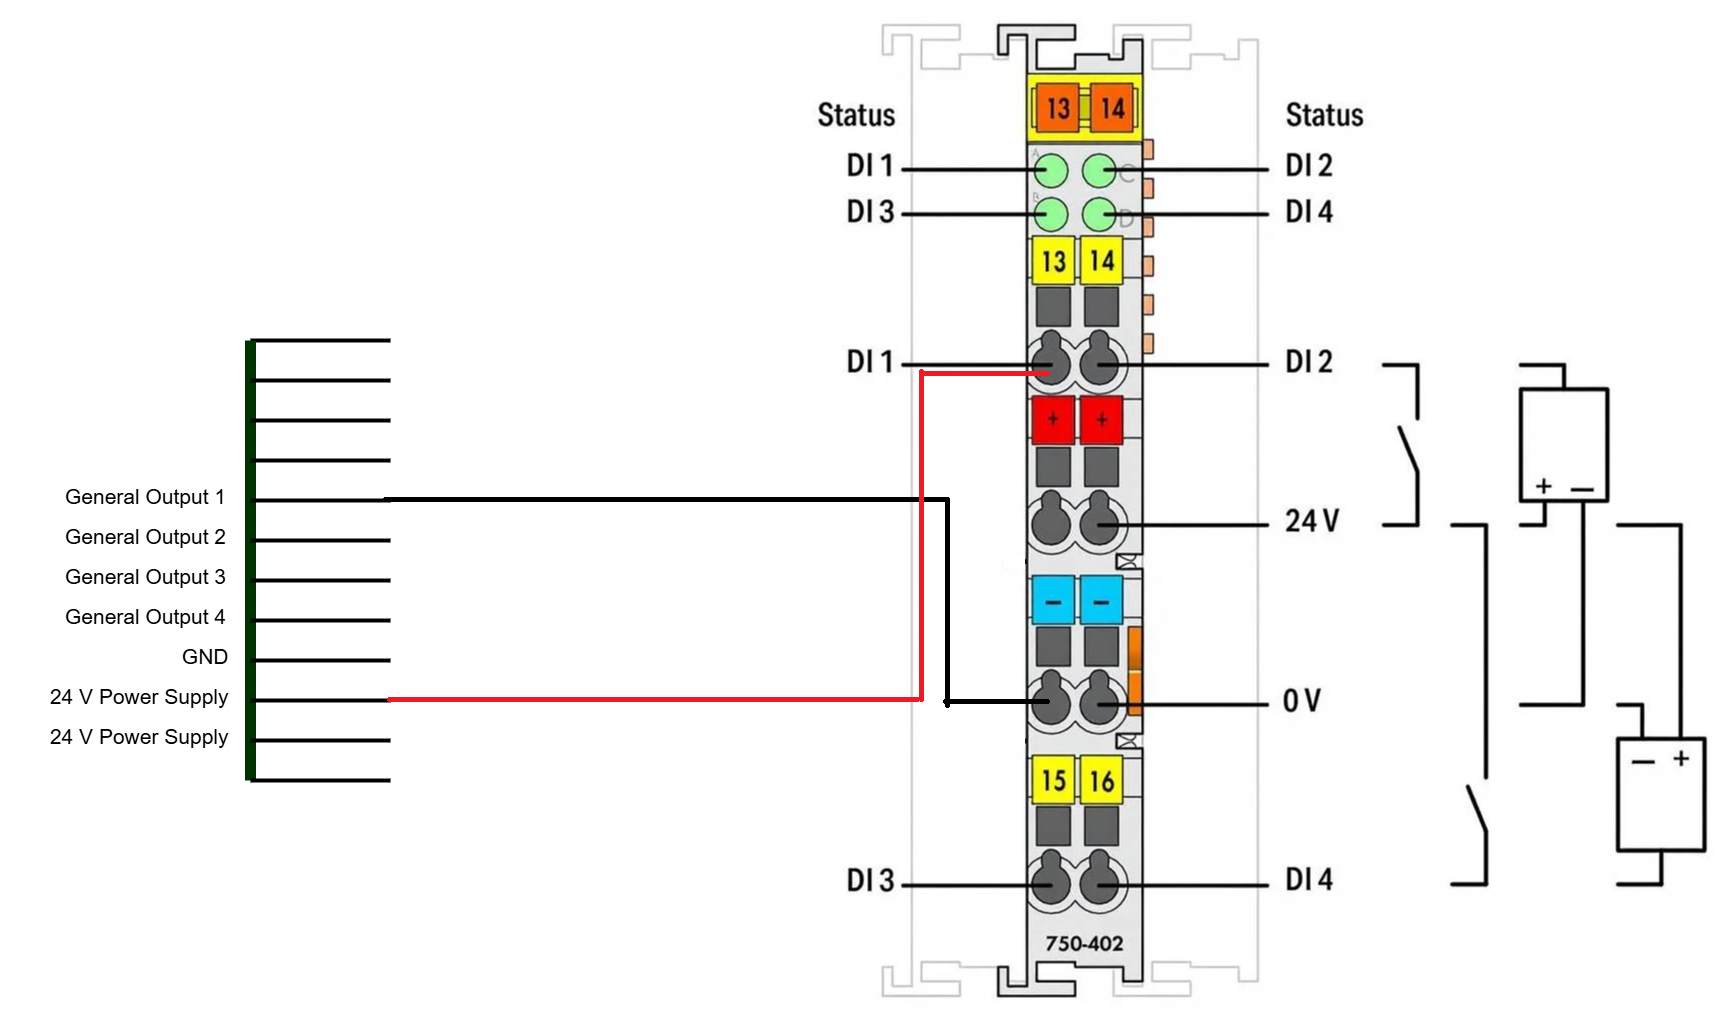
\includegraphics[height=7.4cm]{pic/sewing-machine-plc-init.png}
	\caption{Initial Connection of Sewing Machine to PLC}
	\label{fig:Model-Component-Pattern}
\end{figure}
The resolution of the aforementioned issue necessitated the conversion of the NPN signals of the sewing machine into PNP signals, which are compatible with the PLC. For the execution of this task, an optocoupler was utilized. The implementation was executed in accordance with the subsequent description. Subsequently, the signal output pins of the sewing machine were connected to the signal input connectors of the optocoupler. Furthermore, a connection to the 24-V power supply of the sewing machine was established for each signal input. The signal connectors on the output side of the optocoupler are connected to the signal input connectors of the PLC. Concurrently, the 24-V power supply of the PLC is connected to the VCC input connector of the optocoupler. Additionally, the 0V connector of the programmable logic controller PLC is linked to the GND connector of the optocoupler. The wiring of the optocoupler can be observed in the following Figure.
\begin{figure}[H]
	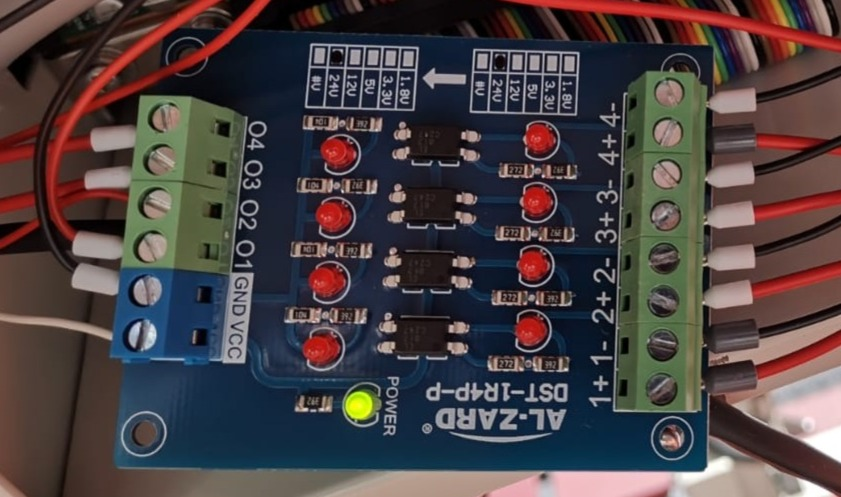
\includegraphics[height=8cm]{pic/optocoupler-wiring.jpg}
	\caption{Initial Connection of Sewing Machine to PLC}
	\label{fig:Model-Component-Pattern}
\end{figure}
As illustrated, the red cables represent electrical connections originating from or terminating at a 24V power source. Additionally, the white cable located on the left side is linked to the 24V source of the PLC. The black cables serve as connections to ground or to the signal pins on the right side. These connections function in a manner that pulls down the current when signals are in a state of activity.


